
\documentclass[norsk,a4paper,12pt]{article}
\usepackage[T1]{fontenc} %for å bruke æøå
\usepackage[utf8]{inputenc}
\usepackage{graphicx} %for å inkludere grafikk
\usepackage{verbatim} %for å inkludere filer med tegn LaTeX ikke liker
\usepackage{mathpazo}
\usepackage{listings}
\bibliographystyle{plain}
\usepackage{xcolor}

\definecolor{background}{gray}{0.95}
\definecolor{comment}{rgb}{0,0.5,0}
\colorlet{keyword}{blue}
\colorlet{string}{red}
\lstset{numbers=left,
	title=\lstname,
	numberstyle=\tiny, 
	breaklines=true,
	tabsize=4,
	language=Python,
	morekeywords={with,super,as},,
	frame=single,
	basicstyle=\footnotesize\tt,
	commentstyle=\color{comment},
	keywordstyle=\color{keyword},
	stringstyle=\color{string},
	backgroundcolor=\color{background},
	showstringspaces=false,
	numbers=left,
	numbersep=5pt,
	literate=
		{æ}{{\ae}}1
		{å}{{\aa}}1
		{ø}{{\o}}1
		{Æ}{{\AE}}1
		{Å}{{\AA}}1
		{Ø}{{\O}}1
	}



\title{Prosjekt}
\author{KANDIDATNUMMER}
\date{\today}
\begin{document}

\maketitle


\section*{Oppgave 1}

Se plot for plot, kode for kode.
\\
\\
\begin{figure}
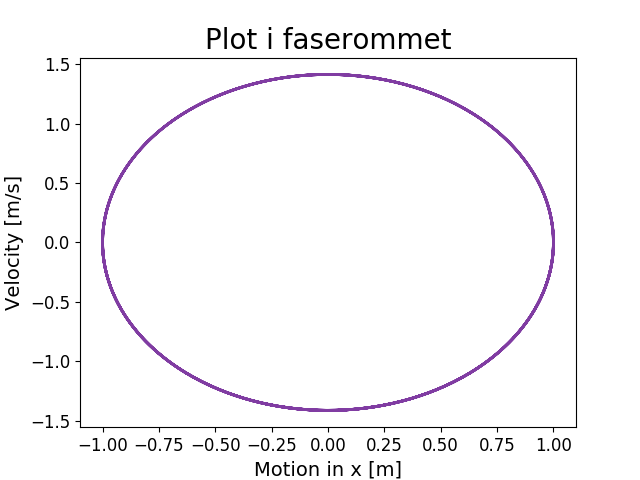
\includegraphics[scale=1]{Oppgave1.png}
\end{figure}
\\
Totalenergien viser et eller annet, FINN UT AV HVA TOTALENERGIEN ER. Siden det ikke er noen form for friksjon så vil energien bare veksle mellom potensiell og kinetisk. + mer forklaring
\\
\\
\\
Hvorfor står banen i faserommet vinkelrett på x og y aksen?
\\
\\
\\
Systemet i faserommet beveger sem med klokka. Det går ikke ann å bruke en kombinasjon av initialverdier til å få den til å gå motsatt retning, fordi det avhenger av hvordan vi har satt positiv retning.  SIKKERT IKKE HELT RIKTIG ELLER KOMPLETT, SÅ DISKUTER LITT OG SKRIV BEDRE




\section*{Oppgave 2}


\begin{figure}
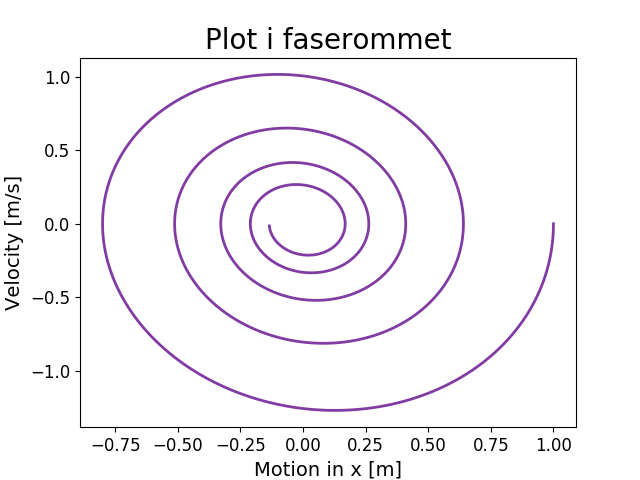
\includegraphics[scale=1]{Oppgave2.png}
\end{figure}


\section*{Oppgave 3}

\section*{Oppgave 4}

\section*{Oppgave 5}

\section*{Oppgave 6}

\section*{Oppgave 7}

\section*{Oppgave 8}

\section*{Oppgave 9}






\end{document}